\documentclass[]{article}
\usepackage{graphicx}

\topmargin=0.0in 
\oddsidemargin=0.0in 
\evensidemargin=0in 
\textwidth=6.5in 
\marginparwidth=0.5in
\headheight=0pt  
\headsep=0pt 
\textheight=9.0in 
\newcommand\tab[1][3cm]{\hspace*{#1}}
\begin{document}
\begin{center}
	{
	
	\Large{\textbf{Shruti Manish Kothadia}}\\
	}
\end{center}

\begin{center}
\vspace{+0.1in}
Flat No.1, Building No.12, Laxminarayan Nagar, Erandwane, Pune-411004.Maharashtra.
\end{center}
\begin{flushleft}
\vspace{-0.1in}
Contact No:+91-8087186701.\hspace{2.7 in} Email: kshruti.3003@gmail.com
\end{flushleft}
\vspace{-0.2in}
\noindent\rule{16.5cm}{0.4pt}


\begin{flushright}
\begin{figure}[h]
\hspace{5.1in}
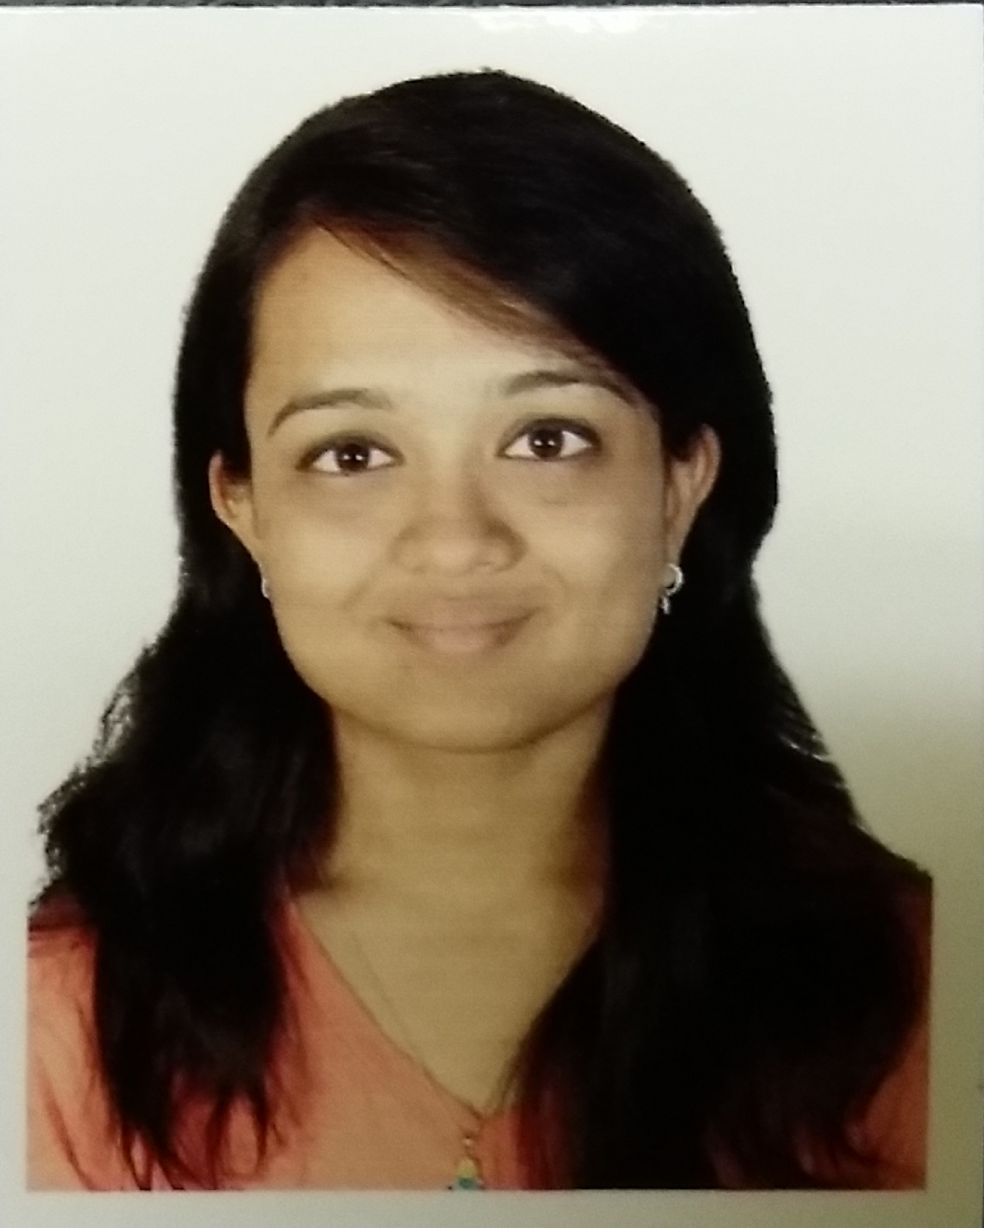
\includegraphics[width=90px]{shruti}

\end{figure}
\end{flushright}
\begin{flushleft}
\vspace{-0.4in}
 	\textbf{\large OBJECTIVE:}
 	\hspace{0.02in}
 	To improve my technical skills by applying them in real life.
  \end{flushleft}
 \begin{flushleft}
 \vspace{0.15in}
  	\textbf{\large EDUCATION:}
 	
 \vspace{0.15in}
 	\begin{tabular}{||l|c|c|c||}
 	\hline 
 	Course & Year & Institute & Percentage \\ 
 	\hline 
 	T.E(ENTC) & 2016 & Pune Institute of Compter Technology & 73.09 \\ 
 	\hline 
 	HSC(Maharashtra State Board) & 2012 & M E S Abasaheb Garware College,Pune & 84.16 \\ 
 	\hline 
 	SSC(Maharashtra State Board) & 2010 & Vidya Pratishthans' Bal Vikas Mandir,Baramati & 93.27 \\ 
 	\hline 
 	\end{tabular} 
 \end{flushleft}
 
 
 \begin{flushleft}	                                  
  \vspace{0.15in}
{\large \bf PROJECTS}                                                                 
 \begin{enumerate}	
 \vspace{-0.1in}	                                 
 \addtolength{\itemindent}{1in}
\item  Landmine Detecting Rover.
\item  Electronic Voting Machine using logic gates.
\end{enumerate}
\end{flushleft}


\begin{flushleft}
\vspace{0.15in}
{\large \bf INTERNSHIP}
\begin{itemize}
\hspace{0.5in}
\vspace{-0.22in}
\addtolength{\itemindent}{1in}
\item Summer Internship at IIT Bombay.
\end{itemize}
\end{flushleft}


\begin{flushleft}
\vspace{0.15in}
{\large \bf TECHNICAL SKILLS}
\begin{itemize}
\hspace{0.5in}
{\bf Programming Languages}
{
\addtolength{\itemindent}{1in}
\item C

\item Embedded C
\item Python\
}

\hspace{0.5in}
{\bf Simulation Softwares}
{
\addtolength{\itemindent}{1in}
\item MATLAB
\item Multisim
\item LabVIEW
\item Keil uVision
\item MPLAB


\item Power Electronics.
\item Arduino
}
\end{itemize}
\end{flushleft}


\begin{flushleft}

\vspace{0.15in}
{\large \bf SOFT SKILLS}
\begin{itemize}
\hspace{0.5in}
\vspace{-0.22in}
\addtolength{\itemindent}{1in}
\item Organised
\item Consistent.
\item Good Listener.
\end{itemize}
\end{flushleft}


\begin{flushleft}
\vspace{0.15in}
{\large \bf EXTRA CURRICULAR ACTIVITIES}
\begin{itemize}
\hspace{0.5in}
\vspace{-0.22in}
\addtolength{\itemindent}{1in}
\item Finance Head in Scientia '15.
\item Digital Design head in Scientia '15.
\item Organizer (Event Head of Ethical Hacking Workshop).
\end{itemize}
\end{flushleft}


\begin{flushleft}
\vspace{0.15in}
{\large \bf CO-CURRICULAR ACTIVITIES}
\begin{itemize}
\hspace{0.5in}
\vspace{-0.22in}
\addtolength{\itemindent}{1in}
\item {\bf Winner} in Circuit Designing and Debugging Competition in Scientia '13.
\item {\bf Winner} in Circuit Designing and Debugging Competition in Credenz '13.
\item {\bf Winner} in Energy Audit Competition.
\item {\bf Winner} in "Closest to Market Category" in e-Yantra Ideas Competition. 
\end{itemize}
\end{flushleft}


\begin{flushleft}
\vspace{0.15in}
{\large \bf PERSONAL INFORMATION}\\
\vspace{0.15in}
Father's Name:
\hspace{0.5in}
Manish Anil Kothadia
\vspace{0.15in}


Mother's Name
\hspace{0.5in}
Supriya Manish Kothadia\\
\vspace{0.15in}
Date of Birth:
\hspace{0.5in}
03/06/1995.
\end{flushleft}


\begin{flushleft}
\vspace{0.15in}
{\large \bf REFERENCE}
\hspace{0.2in}
Google
\end{flushleft}


\begin{flushleft}
\vspace{0.15in}
{\large \bf DECLARATION}\\
\vspace{0.15in}
I hereby declare that the above information is true,correct and complete to the best of my knowledge and belief.
\end{flushleft}


\begin{flushleft}
\vspace{0.15in}
{\large \bf DATE :}
\hspace{0.01in}
25th May 2016
\end{flushleft}
\end{document}